
\section{流动拓扑：置换、混合通风的数学拓扑理解}

\subsection{基本假设}
\begin{itemize}
    \item 输运的主导结构是几何性的，而非耗散性的：房间内的气流结构主要由几何边界和源汇位置决定
    \item 只关心房间通风中的流动拓扑
    \item 如果一个数学结构在极简假设下已经是不可避免的，那么真实物理只会在其上加修饰，而不会推翻它
\end{itemize}
We assume that the global ventilation structure is primarily governed by geometric confinement and mass conservation, and can therefore be captured by an idealized potential-flow representation. Within this framework, the focus is placed on the topological organization of streamlines rather than on dissipative details.

我们假设全局通风结构主要受几何约束和质量守恒的控制，因此可以通过理想化的势流表示来捕捉。在这个框架内，重点放在流线的拓扑组织上，而不是耗散细节上。

\subsection{室内通风问题的数学抽象}
在有界域中，由若干通量源驱动的二维保守输运问题。那么它满足：
\begin{itemize}
    \item Laplace 方程
    \item 复势表示
    \item sc变换
    \item 点源点汇叠加
    \item 流线=物质线
\end{itemize}

\begin{figure}
\centering
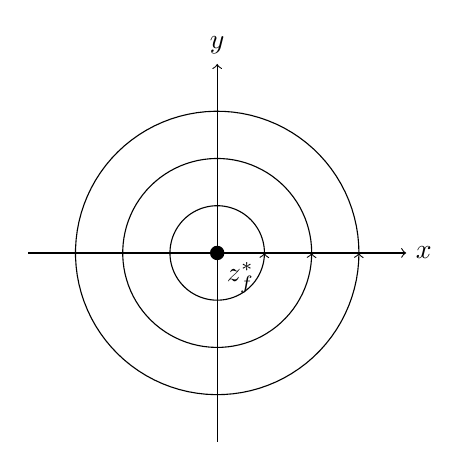
\begin{tikzpicture}[scale=1.2]
\draw[->] (-2,0) -- (2,0) node[right] {$x$};
\draw[->] (0,-2) -- (0,2) node[above] {$y$};

\foreach \r in {0.5,1,1.5}
{
  \draw[->,domain=0:360,samples=100]
  plot ({\r*cos(\x)}, {\r*sin(\x)});
}

\filldraw (0,0) circle (2pt) node[below right] {$z_f^{*}$};
\end{tikzpicture}
\caption{Schematic phase portrait of a stable spiral equilibrium.}
\label{fig:local_phase_portrait}
\end{figure}


黏性不会消灭拓扑结构，只会钝化它

